
\section{Building the asymmetric unit}
\label{buildingunitcell}

Once we have selected the $models$ for \ttt{metHgb} $\alpha$ and $\beta$ subunits (see the workflow branches to have $\alpha$ and $\beta$ subunits \ffigure{fig:scipion_workflow_whole_reconstruction}), we can regenerate the smallest asymmetrical element of the starting map. With this aim we are going to use protocols to operate with atomic structures (\scommand{chimerax - operate} or \scommand{atomstructutils - operator}), to refine them both manually (\scommand{ccp4 - coot refinement}) and automatically (\scommand{phenix - real space refine}) and to validate them (\scommand{phenix - validation\_cryoem} and \scommand{phenix - emringer}). A brief schema of the main steps of this part of the workflow can be seen in \ffigure{fig:scipion_workflow_whole_reconstruction}. Take into account that in real live probably many more steps of refinement and validation will be required.\\ 

 \begin{figure}[H]
  \centering 
  \captionsetup{width=.9\linewidth} 
  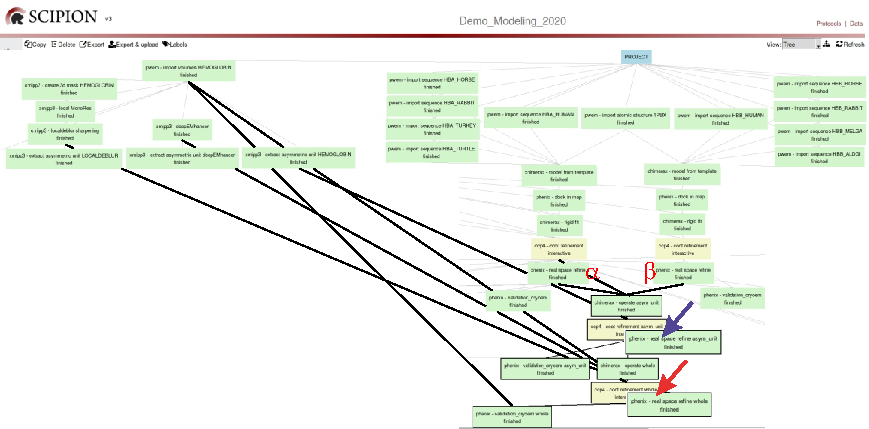
\includegraphics[width=1\textwidth]{Images/Fig73}
  \caption{\scipion framework detailing the workflow to reconstruct the structure of the map asymmetric unit (blue arrow) and the whole atomic structure (red arrow).}
  \label{fig:scipion_workflow_whole_reconstruction}
  \end{figure}

\begin{itemize}
 \item Protocol to join the \ttt{metHgb} $\alpha$ and $\beta$ subunits in a unique atomic structure:\\ Two protocols can be used in \scipion for this purpose (\scommand{chimerax - operate} or \scommand{atomstructutils - operator}) and the result should be identical. \\
 Before starting, nevertheless, be sure that you have two atomic structures and each one includes an only chain with a different name. Remember that chain names should have changed for other chain names than the first one before saving the refined atomic structure in \coot (\ffigure{fig:chimerax_asymm_unit_2}). There is an additional way of modifying chain names in \chimera using the \chimera command lines (to change chain A to chain B in model \ttt{\#2}):\\ \ttt{setattr \#2/A c chain\_id B}\\ \ttt{setattr \#2/A r chain\_id B}\\ \ttt{scipionwrite \#2 prefix chainAtoB\_}\\Secondly, it could be very convenient to change the \scipion output label of each subunit, in order to follow them easily in \scipion. According to the \ffigure{fig:scipion_workflow_edition} go to the Summary of the two final protocols that allow to generate those atomic structures and press the black arrow (C) to select the option \ttt{Edit}. Type the new output name of the structures (\ttt{HBA\_refined} (D) and \ttt{HBB\_refined} (E), respectively).\\
    
  \begin{figure}[H]
  \centering 
  \captionsetup{width=.9\linewidth} 
  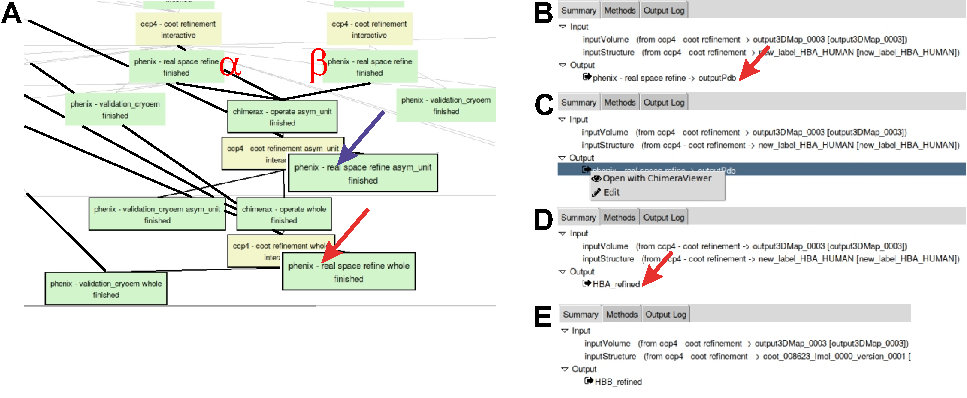
\includegraphics[width=1\textwidth]{Images/Fig75}
  \caption{A. Zoom in on \ffigure{fig:scipion_workflow_whole_reconstruction}. B. Summary of the protocol box from \phenix \ttt{real space refine} ($\alpha$ in (A)). Red arrow points at the \scipion output name. C. Menu opened pressing the output black arrow of the Summary. D. New name of the \scipion output in the Summary. E. Summary from the protocol box \phenix \ttt{real space refine} ($\beta$) after applying the same edition process.}
  \label{fig:scipion_workflow_edition}
  \end{figure}
  
  Then, open again $ChimeraX$ \ttt{operate} protocol and following the already indicated instructions, include the $models$ of \ttt{metHgb} $\alpha$ and $\beta$ subunits in params \ttt{Atomic structure} and \ttt{Other atomic structures}, respectively (\ffigure{fig:chimerax_asymm_unit_1} (A)). Firstly, check that both \ttt{models} are perfectly fitted in the map asymmetric unit. Otherwise, apply the command \ttt{fitmap}, as it was previously shown. Next, create a single atomic structure by joining models \ttt{\#3} and \ttt{\#4} in $ChimeraX$ \ttt{Models} panel. To generate a combined \ttt{model} write in the command line:\\
  \\ \ttt{scipioncombine \#3,4}\\
  \\The new model \ttt{\#5} is shown in $ChimeraX$ \ttt{Models} panel (\ffigure{fig:chimerax_asymm_unit_1}). Finally, save this fitted structure writing in $ChimeraX$ command line:\\ 
  \\ \ttt{scipionwrite \#5 prefix asymmetric\_unit\_model\_}\\ 
    
  \begin{figure}[H]
  \centering 
  \captionsetup{width=.9\linewidth} 
  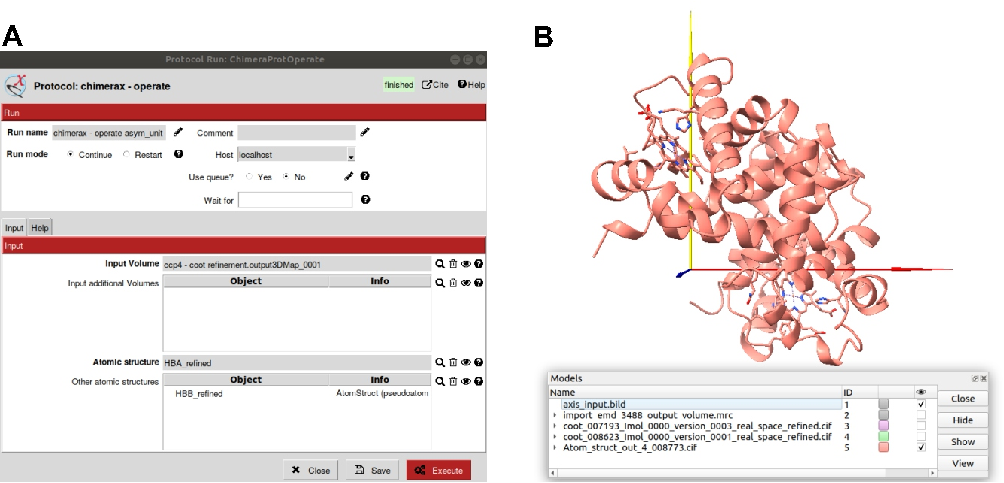
\includegraphics[width=1\textwidth]{Images/Fig76}
  \caption{A. Completing the \scommand{chimerax - operate} protocol with the atomic structures \ttt{HBA\_refined} and \ttt{HBB\_refined} . B. \chimera graphics window showing the combined \ttt{model \#5}.}
  \label{fig:chimerax_asymm_unit_1}
  \end{figure}

 \item Protocols to refine the new combined structure generated:\\
  
At this point refinements could cover specially the overlapping area between the two chains. Help yourself with the \coot tools of \ttt{Validate} in the main menu, as well as the visualization tools of \phenix \ttt{real space refine} protocol. 
 \item Validation protocols to select the best $model$ of the human \ttt{metHgb} unit cell:\\
 \\Validate the new combined structure generated is recommendable before continuing with the next steps in the workflow.$EMRinger$ and $Validation CryoEM (MolProbity)$ validation statistics should be computed for the new $model$ of human \ttt{metHgb} asymmetric unit, generated by combining \ttt{metHgb} $\alpha$ and $\beta$ subunits. Appendix \ref{app:solutions} (\textbf{Question \ref{buildingunitcell}\_1}) contains a statistics table for the unit cell $model$ (\ttable{table:refmac_question_11}). We can try to improve those statistics by additional refinement processes. By performing refinement in real space with $Phenix$ some of the statistics could result improved. \ttable{table:refmac_question_11} contains also RMSD values computed in a similar way as we have seen for $\alpha$ and $\beta$ subunits, considering as fixed structure chains A and B from \ttt{5NI1} atomic structure. To continue with the modeling process we can select the unit cell $model$ generated by $Phenix$ \ttt{real space refine} because most of its validation statistics show the best values (\ccmask, $EMRinger$ \ttt{score} and $MolProbity$ values). Exceptionally, RMSD regarding the published structure yields the worst value.
 
\end{itemize}

